\documentclass[border=1]{standalone}
\usepackage{tikz}

\usetikzlibrary{decorations.markings, arrows}

\tikzset{
    point/.style={ draw, scale=0.15, color=black!50, circle, fill },
    line/.style={ draw, -latex, decoration={
    markings,
    mark=at position 0.1 with {\arrow{{stealth}}}} },
    polygon/.style={ white, solid, fill=black!08 }
}

\begin{document}
    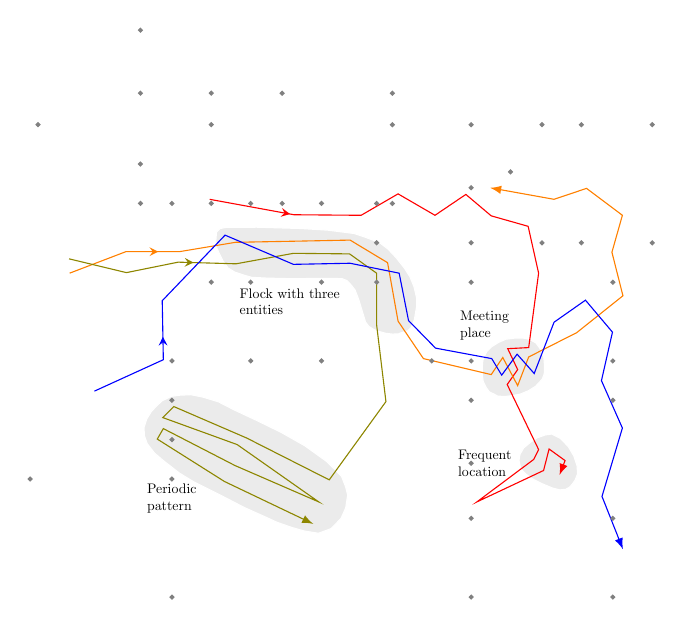
\begin{tikzpicture}
        \draw[polygon] (2.002, 4.181) -- (1.956, 4.135) -- (1.949, 4.041) -- (1.949, 3.957) -- (1.991, 3.866) -- (2.04, 3.768) -- (2.103, 3.68) -- (2.187, 3.628) -- (2.306, 3.589) -- (2.404, 3.561) -- (2.6, 3.551) -- (2.905, 3.544) -- (3.237, 3.547) -- (3.461, 3.547) -- (3.552, 3.544) -- (3.615, 3.519) -- (3.667, 3.463) -- (3.716, 3.4) -- (3.762, 3.281) -- (3.849, 2.994) -- (3.891, 2.938) -- (3.947, 2.903) -- (4.003, 2.879) -- (4.101, 2.851) -- (4.192, 2.84) -- (4.269, 2.844) -- (4.311, 2.861) -- (4.385, 2.882) -- (4.427, 2.921) -- (4.469, 3.022) -- (4.497, 3.187) -- (4.497, 3.302) -- (4.465, 3.439) -- (4.413, 3.568) -- (4.343, 3.677) -- (4.238, 3.81) -- (4.136, 3.918) -- (4.028, 4.002) -- (3.849, 4.069) -- (3.702, 4.118) -- (3.374, 4.16) -- (3.034, 4.181) -- (2.467, 4.198) -- (2.075, 4.195) -- (2.002, 4.181) -- cycle;
\draw[polygon] (1.484, 2.064) -- (1.383, 2.05) -- (1.267, 1.994) -- (1.194, 1.927) -- (1.127, 1.854) -- (1.071, 1.763) -- (1.036, 1.654) -- (1.04, 1.553) -- (1.075, 1.451) -- (1.169, 1.329) -- (1.281, 1.234) -- (1.488, 1.073) -- (1.666, 0.965) -- (2.002, 0.797) -- (2.313, 0.636) -- (2.555, 0.528) -- (2.723, 0.451) -- (2.915, 0.384) -- (3.073, 0.339) -- (3.251, 0.311) -- (3.412, 0.37) -- (3.538, 0.5) -- (3.597, 0.633) -- (3.622, 0.797) -- (3.597, 0.898) -- (3.545, 1.031) -- (3.472, 1.108) -- (3.349, 1.227) -- (3.076, 1.423) -- (2.772, 1.595) -- (2.464, 1.745) -- (2.18, 1.878) -- (1.981, 1.98) -- (1.788, 2.039) -- (1.631, 2.071) -- (1.484, 2.064) -- cycle;
\draw[polygon] (5.749, 2.79) -- (5.631, 2.775) -- (5.539, 2.735) -- (5.445, 2.676) -- (5.39, 2.62) -- (5.358, 2.556) -- (5.338, 2.504) -- (5.331, 2.407) -- (5.331, 2.34) -- (5.342, 2.243) -- (5.379, 2.165) -- (5.421, 2.106) -- (5.48, 2.079) -- (5.53, 2.051) -- (5.631, 2.049) -- (5.716, 2.06) -- (5.812, 2.077) -- (5.922, 2.123) -- (6.009, 2.178) -- (6.092, 2.267) -- (6.119, 2.335) -- (6.121, 2.447) -- (6.114, 2.541) -- (6.062, 2.661) -- (6.011, 2.729) -- (5.933, 2.773) -- (5.867, 2.788) -- (5.749, 2.79) -- cycle;
\draw[polygon] (6.214, 1.571) -- (6.133, 1.56) -- (6.03, 1.523) -- (5.945, 1.468) -- (5.857, 1.394) -- (5.809, 1.311) -- (5.798, 1.234) -- (5.814, 1.158) -- (5.833, 1.116) -- (5.884, 1.064) -- (5.936, 1.022) -- (5.993, 0.989) -- (6.08, 0.945) -- (6.152, 0.915) -- (6.227, 0.884) -- (6.317, 0.862) -- (6.391, 0.869) -- (6.441, 0.897) -- (6.476, 0.937) -- (6.509, 0.983) -- (6.542, 1.066) -- (6.535, 1.169) -- (6.494, 1.293) -- (6.424, 1.411) -- (6.323, 1.516) -- (6.214, 1.571) -- cycle;

        \draw[line, color=red, postaction={decorate}] (1.869, 4.552) -> (2.94, 4.356) -- (3.793, 4.349) -- (4.262, 4.621) -- (4.731, 4.349) -- (5.123, 4.614) -- 
(5.445, 4.342) -- (5.914, 4.209) -- (6.047, 3.614) -- (5.921, 2.669) -- (5.655, 2.655) -- (5.781, 2.389) -- (5.648, 2.2) -- (6.047, 1.374) -- (5.984, 1.248) -- 
(5.263, 0.709) -- (6.11, 1.108) -- (6.18, 1.381) -- (6.383, 1.234) -- (6.313, 1.052);
\draw[line, color=orange, postaction={decorate}] (0.091, 3.614) -- (0.805, 3.887) -- (1.484, 3.887) -- (2.198, 4.006) -- (2.947, 4.02) -- (3.653, 4.034) -- 
(4.129, 3.747) -- (4.262, 3.005) -- (4.584, 2.529) -- (5.445, 2.326) -- (5.592, 2.543) -- (5.781, 2.186) -- (5.921, 2.55) -- (6.53, 2.858) -- (7.118, 3.327) -- 
(6.978, 3.88) -- (7.111, 4.349) -- (6.656, 4.691) -- (6.243, 4.552) -- (5.431, 4.698);
\draw[line, color=olive, postaction={decorate}] (0.084, 3.796) -- (0.812, 3.621) -- (1.47, 3.754) -- (2.205, 3.733) -- (2.933, 3.866) -- (3.646, 3.859) -- 
(3.989, 3.614) -- (3.989, 2.963) -- (4.108, 1.983) -- (3.388, 0.989) -- (2.338, 1.521) -- (1.414, 1.92) -- (1.274, 1.78) -- (2.219, 1.437) -- (3.255, 0.709) -- 
(2.191, 1.171) -- (1.281, 1.64) -- (1.204, 1.507) -- (2.058, 0.968) -- (3.185, 0.43);
\draw[line, color=blue, postaction={decorate}] (0.406, 2.116) -- (1.281, 2.515) -- (1.267, 3.264) -- (2.065, 4.097) -- (2.933, 3.726) -- (3.653, 3.74) -- 
(4.276, 3.614) -- (4.395, 3.012) -- (4.738, 2.662) -- (5.452, 2.529) -- (5.578, 2.319) -- (5.774, 2.585) -- (5.991, 2.34) -- (6.243, 2.991) -- (6.642, 3.271) -- 
(6.985, 2.865) -- (6.845, 2.249) -- (7.111, 1.647) -- (6.852, 0.779) -- (7.118, 0.108);

        \node[point] at (-0.31, 5.5) {};
%\node[point] at (0.49, 4.5) {};
%\node[point] at (0.49, 4.0) {};
\node[point] at (0.99, 6.7) {};
\node[point] at (0.99, 5.9) {};
\node[point] at (0.99, 5.0) {};
\node[point] at (0.99, 4.5) {};
\node[point] at (1.89, 5.9) {};
\node[point] at (1.89, 5.5) {};
\node[point] at (1.89, 4.5) {};
\node[point] at (1.39, 4.5) {};
\node[point] at (1.39, 1.5) {};
\node[point] at (1.39, 2.0) {};
\node[point] at (1.39, 2.5) {};
\node[point] at (1.39, 1.0) {};
\node[point] at (1.39, -0.5) {};
\node[point] at (-0.41, 1.0) {};
%\node[point] at (0.49, 1.5) {};
%\node[point] at (0.49, 2.0) {};
\node[point] at (1.89, 3.5) {};
%\node[point] at (2.39, 3.9) {};
\node[point] at (2.39, 4.5) {};
\node[point] at (2.39, 3.5) {};
\node[point] at (2.39, 2.5) {};
\node[point] at (2.79, 5.9) {};
\node[point] at (2.79, 4.5) {};
%\node[point] at (2.79, 3.9) {};
\node[point] at (3.29, 4.5) {};
%\node[point] at (3.29, 3.9) {};
\node[point] at (3.29, 3.5) {};
\node[point] at (3.29, 2.5) {};
\node[point] at (3.99, 3.5) {};
\node[point] at (3.99, 4.0) {};
\node[point] at (3.99, 4.5) {};
\node[point] at (5.19, 4.0) {};
\node[point] at (5.19, 3.5) {};
\node[point] at (5.19, 2.5) {};
\node[point] at (5.19, 2.0) {};
\node[point] at (5.19, 1.2) {};
\node[point] at (5.19, 0.5) {};
\node[point] at (6.99, 3.5) {};
\node[point] at (6.99, 2.5) {};
\node[point] at (6.99, 2.0) {};
\node[point] at (6.99, 0.5) {};
\node[point] at (6.99, -0.5) {};
\node[point] at (5.19, -0.5) {};
\node[point] at (6.09, 4.0) {};
\node[point] at (6.59, 4.0) {};
\node[point] at (7.49, 4.0) {};
\node[point] at (7.49, 5.5) {};
\node[point] at (6.59, 5.5) {};
\node[point] at (6.09, 5.5) {};
%\node[point] at (6.09, 5.0) {};
\node[point] at (5.19, 4.7) {};
\node[point] at (5.69, 4.9) {};
\node[point] at (5.19, 5.5) {};
\node[point] at (4.19, 5.5) {};
\node[point] at (4.19, 4.5) {};
\node[point] at (4.19, 5.9) {};
\node[point] at (4.69, 2.5) {};
%\node[point] at (4.69, 3.5) {};

        
        \node[scale=0.5, text width=3cm] at (3.00,3.25){Flock with three entities};
        \node[scale=0.5, text width=1cm] at (5.30,2.95){Meeting place};
        \node[scale=0.5, text width=1.5cm] at (5.40,1.20){Frequent location};
        \node[scale=0.5, text width=1.5cm] at (1.45,0.75){Periodic pattern};
    \end{tikzpicture}
\end{document}
